\documentclass[aspectratio=1610,8pt]{beamer}

% Theme and color scheme
\usetheme{Madrid}
\usecolortheme{whale}

% Simplified 3-color palette (Navy Blue, Steel Blue, Light Gray)
\definecolor{navyblue}{RGB}{25,50,125}
\definecolor{steelblue}{RGB}{70,130,180}
\definecolor{lightgray}{RGB}{240,240,240}

% Custom color settings
\setbeamercolor{structure}{fg=navyblue}
\setbeamercolor{frametitle}{bg=navyblue,fg=white}
\setbeamercolor{title}{fg=navyblue}
\setbeamercolor{block title}{bg=steelblue,fg=white}
\setbeamercolor{block body}{bg=lightgray}
\setbeamercolor{block title alerted}{bg=navyblue,fg=white}
\setbeamercolor{block body alerted}{bg=lightgray}

% Packages
\usepackage{graphicx}
\usepackage{amsmath,amssymb,amsfonts}
\usepackage{booktabs}
\usepackage{subcaption}
\usepackage{multicol}
\usepackage{xcolor}
\usepackage{colortbl}
\usepackage{tikz}
\usepackage{tcolorbox}

% Enhanced spacing and formatting
\setlength{\parskip}{2pt}
\setbeamertemplate{itemize items}[circle]
\setbeamertemplate{enumerate items}[default]
\setbeamertemplate{navigation symbols}{}

% Simplified highlighting commands
\newcommand{\highlight}[1]{\textcolor{navyblue}{\textbf{#1}}}
\newcommand{\emphasis}[1]{\textcolor{steelblue}{\textbf{#1}}}

% Title information
\title{Image Types, Storage Formats, Coding \& Compression}
\subtitle{CMSC 178IP - Digital Image Processing}
\author{Noel Jeffrey Pinton}
\institute{Department of Computer Science\\University of the Philippines - Cebu}
\date{\today}

\begin{document}

% Title Slide
\begin{frame}
\titlepage
\begin{center}
\vspace{0.5cm}
\begin{tcolorbox}[colback=lightgray,colframe=navyblue,width=0.8\textwidth,center,boxrule=1pt]
\centering
\textbf{Understanding Digital Image Fundamentals}\\
\textit{From Raw Pixels to Optimized Storage Solutions}
\end{tcolorbox}
\end{center}
\end{frame}

% Learning Objectives Slide
\begin{frame}{Today's Learning Objectives}
\begin{columns}[T]
\column{0.5\textwidth}
\begin{alertblock}{\highlight{Core Concepts}}
\textbf{Image Types:} Binary, grayscale, color, indexed

\textbf{Bit Depth:} 1-bit, 8-bit, 16-bit, 24-bit systems

\textbf{Color Models:} RGB, CMYK, HSV representations

\textbf{Resolution:} Spatial vs. intensity resolution
\end{alertblock}

\textbf{Real-world Applications:}
\begin{itemize}
    \item Web graphics, mobile photography
    \item Medical imaging systems
    \item Satellite imagery processing
    \item Social media platforms
\end{itemize}

\column{0.5\textwidth}
\begin{alertblock}{\highlight{Storage \& Compression}}
\textbf{Formats:} BMP, JPEG, PNG, GIF, TIFF

\textbf{Compression:} Lossless vs. lossy techniques

\textbf{Algorithms:} Huffman, LZW, DCT, wavelets

\textbf{Trade-offs:} Quality vs. file size analysis
\end{alertblock}

\begin{center}
\vspace{0.5cm}
\begin{tcolorbox}[colback=steelblue,colframe=steelblue,width=0.9\textwidth,center,boxrule=1pt]
\centering
\textcolor{white}{\textbf{From raw pixels to optimized storage solutions!}}
\end{tcolorbox}
\end{center}

\end{columns}
\end{frame}

% Course Context Slide
\begin{frame}{Course Context - Where We Are}
\begin{center}
\textbf{Digital Image Processing Pipeline}
\end{center}

\begin{center}
\begin{tabular}{|c|c|c|c|c|}
\hline
Raw Image & \cellcolor{steelblue}\textcolor{white}{Image Types} & Enhancement & Analysis & Applications \\
Capture & \cellcolor{steelblue}\textcolor{white}{\& Storage} & & & \\
\hline
Sensors & Formats & Filtering & Feature & Recognition \\
CCD/CMOS & Compression & Correction & Detection & AI \\
\hline
\end{tabular}
\end{center}

\vspace{0.5cm}
\textbf{Key Questions We'll Answer Today:}
\begin{itemize}
    \item How are different image types represented in memory?
    \item What are the advantages/disadvantages of each storage format?
    \item How do compression algorithms reduce file sizes?
    \item When should we use lossless vs. lossy compression?
\end{itemize}

\begin{center}
\textcolor{steelblue}{\textit{Foundation knowledge for all subsequent image processing techniques}}
\end{center}
\end{frame}

% Digital Image Definition Slide
\begin{frame}{What is a Digital Image?}
\begin{columns}[T]
\column{0.6\textwidth}
\begin{alertblock}{Comprehensive Definition}
A digital image is a \textbf{2D array of pixels} (picture elements), where each pixel contains discrete intensity values representing color or brightness information at specific spatial locations.
\end{alertblock}

\textbf{Mathematical Foundation:}
\begin{itemize}
    \item Image function: $f(x, y)$
    \item Spatial coordinates: $x \in [0, M-1], y \in [0, N-1]$
    \item Intensity levels: $L = 2^k$ (k = bit depth)
    \item Pixel values: $0 \leq f(x,y) \leq L-1$
\end{itemize}

\textbf{Digital Characteristics:}
\begin{itemize}
    \item \emphasis{Discrete}: Finite pixel locations
    \item \emphasis{Quantized}: Limited intensity levels
    \item \emphasis{Rectangular}: Grid-based sampling
    \item \emphasis{Finite}: Bounded image dimensions
\end{itemize}

\column{0.4\textwidth}
\textbf{Common Bit Depths \& Ranges:}
\begin{itemize}
    \item \textbf{1-bit}: Binary (0-1)\\
          File size = $M \times N$ bits
    \item \textbf{8-bit}: Grayscale (0-255)\\
          File size = $M \times N$ bytes
    \item \textbf{24-bit}: RGB Color (0-16.7M colors)\\
          File size = $3 \times M \times N$ bytes
\end{itemize}

\begin{center}
\begin{tcolorbox}[colback=navyblue,colframe=navyblue,width=0.9\textwidth,center,boxrule=1pt]
\centering
\textcolor{white}{\textbf{File Size = M $\times$ N $\times$ bit depth $\div$ 8 bytes}}
\end{tcolorbox}
\end{center}

\end{columns}
\end{frame}

% Image Types Classification Slide
\begin{frame}{Image Types - Detailed Classification}
\begin{center}
\textbf{Four Main Image Categories}
\end{center}

\begin{center}

\includegraphics[width=0.95\textwidth]{images/image_types_comparison.png}
\end{center}

\begin{columns}[T]
\column{0.5\textwidth}
\textbf{1. Binary Images (1-bit)}
\begin{itemize}
    \item Values: 0 (black), 1 (white)
    \item Applications: OCR, barcode scanning
    \item Size: Smallest storage requirement
    \item Processing: Fast logical operations
\end{itemize}

\textbf{2. Grayscale Images (8-16 bit)}
\begin{itemize}
    \item 8-bit: 256 gray levels (0-255)
    \item 16-bit: 65,536 levels (medical imaging)
    \item Applications: X-rays, scientific imaging
    \item Size: 1/3 of equivalent color image
\end{itemize}

\column{0.5\textwidth}
\textbf{3. Color Images (24-32 bit)}
\begin{itemize}
    \item RGB: 8 bits per channel (16.7M colors)
    \item RGBA: Additional alpha channel
    \item Applications: Photography, web graphics
    \item Size: Largest uncompressed storage
\end{itemize}

\textbf{4. Indexed Color (8-bit)}
\begin{itemize}
    \item Palette-based: 256 colors max
    \item Color lookup table (CLUT)
    \item Applications: GIF animations, icons
    \item Size: Reduced color palette efficiency
\end{itemize}
\end{columns}

\vspace{0.5cm}
\begin{center}
\textcolor{steelblue}{\textbf{Selection depends on application requirements: quality, storage, processing speed}}
\end{center}
\end{frame}

% Binary Images Detail Slide
\begin{frame}{Binary Images - Detailed Analysis}
\begin{columns}[T]
\column{0.6\textwidth}
\begin{alertblock}{\highlight{Definition \& Characteristics}}
Binary images contain only \textbf{two intensity values}: 0 (black) and 1 (white). Each pixel requires exactly \textbf{1 bit} of storage.
\end{alertblock}

\textbf{Technical Specifications:}
\begin{itemize}
    \item Pixel values: $f(x,y) \in \{0, 1\}$
    \item Storage: $\frac{M \times N}{8}$ bytes
    \item Memory efficiency: 8:1 vs grayscale
    \item Bit packing: 8 pixels per byte
\end{itemize}

\textbf{Creation Methods:}
\begin{itemize}
    \item \textbf{Thresholding}: $f(x,y) = \begin{cases} 1 & \text{if } g(x,y) > T \\ 0 & \text{otherwise} \end{cases}$
    \item \textbf{Dithering}: Floyd-Steinberg algorithm
    \item \textbf{Edge detection}: Canny, Sobel operators
\end{itemize}

\column{0.4\textwidth}
\textbf{Applications:}
\begin{itemize}
    \item OCR systems
    \item Barcode reading
    \item Medical bone analysis
    \item Industrial inspection
\end{itemize}

\vspace{0.5cm}
\begin{block}{\emphasis{Trade-offs}}
\textbf{Advantages:}
\begin{itemize}
    \item Fast processing
    \item Minimal storage
    \item Simple algorithms
\end{itemize}

\textbf{Disadvantages:}
\begin{itemize}
    \item Loss of detail
    \item Limited applications
    \item Threshold sensitivity
\end{itemize}
\end{block}

\end{columns}
\end{frame}

% Grayscale Images Detail Slide
\begin{frame}{Grayscale Images - Comprehensive Analysis}
\begin{columns}[T]
\column{0.6\textwidth}
\begin{alertblock}{\highlight{Definition \& Representation}}
Grayscale images represent intensity using shades of gray, typically \textbf{8-bit} (256 levels) or \textbf{16-bit} (65,536 levels).
\end{alertblock}

\textbf{Bit Depth Comparison:}
\begin{itemize}
    \item \textbf{8-bit}: 0-255, standard photography
    \item \textbf{12-bit}: 0-4095, digital cameras
    \item \textbf{16-bit}: 0-65535, scientific imaging
    \item \textbf{32-bit}: Floating point, HDR
\end{itemize}

\vspace{0.3cm}
\begin{center}

\includegraphics[width=0.9\textwidth]{images/bit_depth_comparison.png}
\end{center}

\textbf{RGB Conversion:}
\begin{itemize}
    \item \textbf{Luminance}: $Y = 0.299R + 0.587G + 0.114B$
    \item \textbf{Average}: Gray = $\frac{R+G+B}{3}$
\end{itemize}

\column{0.4\textwidth}
\textbf{Applications:}
\begin{itemize}
    \item Medical X-rays
    \item Satellite imagery
    \item Security systems
    \item Scientific imaging
\end{itemize}

\vspace{0.5cm}
\begin{center}
\begin{tcolorbox}[colback=steelblue,colframe=steelblue,width=0.9\textwidth,center,boxrule=1pt]
\centering
\textcolor{white}{\textbf{Storage: M$\times$N bytes (8-bit)}}\\
\textcolor{white}{\textit{Critical for scientific applications}}
\end{tcolorbox}
\end{center}

\end{columns}
\end{frame}

% RGB Color Model Slide
\begin{frame}{Color Images - RGB Color Model Analysis}
\begin{columns}[T]
\column{0.6\textwidth}
\begin{alertblock}{\highlight{RGB Fundamentals}}
RGB uses \textbf{additive color mixing} with Red, Green, Blue channels. Standard: \textbf{24-bit color} (8 bits per channel).
\end{alertblock}

\textbf{Technical Specifications:}
\begin{itemize}
    \item Each channel: 0-255 (8-bit)
    \item Total colors: $256^3 = 16,777,216$
    \item Storage: $3 \times M \times N$ bytes
    \item Memory layout: Interleaved/planar
\end{itemize}

\textbf{Extended Formats:}
\begin{itemize}
    \item \textbf{RGB565}: Mobile displays (16-bit)
    \item \textbf{RGB888}: Standard 24-bit
    \item \textbf{ARGB8888}: 32-bit with alpha
    \item \textbf{RGB48}: Professional (16-bit/channel)
\end{itemize}

\textbf{Gamma Correction:} $V_{out} = V_{in}^{\gamma}$ where $\gamma \approx 2.2$

\column{0.4\textwidth}
\begin{center}
\textbf{Color Spaces \& Channels}
\end{center}

\begin{center}

\includegraphics[width=0.95\textwidth]{images/color_spaces_demo.png}
\end{center}

\vspace{0.5cm}
\begin{block}{\emphasis{Trade-offs}}
\textbf{Advantage:} Direct display compatibility

\textbf{Challenge:} Large file sizes
\end{block}

\end{columns}
\end{frame}

% Alternative Color Models Slide
\begin{frame}{Alternative Color Models - Beyond RGB}
\begin{columns}[T]
\column{0.5\textwidth}
\textbf{CMYK (Subtractive Model):}
\begin{itemize}
    \item Channels: Cyan, Magenta, Yellow, Black
    \item Application: Printing industry
    \item Color mixing: Ink absorption
    \item Smaller gamut than RGB
\end{itemize}

\textbf{HSV/HSB (Perceptual Model):}
\begin{itemize}
    \item Hue: Color wheel (0-360$^\circ$)
    \item Saturation: Purity (0-100\%)
    \item Value: Brightness (0-100\%)
    \item Intuitive color selection
\end{itemize}

\textbf{Specialized Spaces:}
\begin{itemize}
    \item \textbf{YUV}: Video compression (luminance/chrominance)
    \item \textbf{LAB}: Perceptually uniform
    \item \textbf{XYZ}: CIE standard foundation
\end{itemize}

\column{0.5\textwidth}
\textbf{RGB to HSV:}
$$V = \max(R, G, B)$$
$$S = \frac{V - \min(R,G,B)}{V}$$

\vspace{0.5cm}
\begin{center}
\begin{tcolorbox}[colback=lightgray,colframe=navyblue,width=0.9\textwidth,center,boxrule=1pt]
\textbf{Model Selection:}
\begin{itemize}
    \item \textbf{Display}: RGB color model
    \item \textbf{Print}: CMYK color model
    \item \textbf{Perception}: HSV color model
    \item \textbf{Compression}: YUV color model
\end{itemize}
\end{tcolorbox}
\end{center}

\end{columns}
\end{frame}

% Indexed Color Slide
\begin{frame}{Indexed Color \& Palette Systems}
\begin{columns}[T]
\column{0.6\textwidth}
\begin{alertblock}{\highlight{Concept \& Implementation}}
Indexed color uses a \textbf{Color Lookup Table (CLUT)} with limited colors. Each pixel stores an \textbf{index} (8-bit) to the palette.
\end{alertblock}

\textbf{Technical Structure:}
\begin{itemize}
    \item Pixel values: 0-255 (indices)
    \item Palette: Up to 256 colors
    \item Storage: $M \times N + 256 \times 3$ bytes
    \item Effective when colors < 256
\end{itemize}

\textbf{Palette Algorithms:}
\begin{itemize}
    \item \textbf{Median Cut}: Recursive division
    \item \textbf{Octree}: Tree-based quantization
    \item \textbf{K-means}: Color space clustering
\end{itemize}

\column{0.4\textwidth}
\textbf{Applications:}
\begin{itemize}
    \item GIF animations
    \item Retro games
    \item Scientific visualization
    \item Embedded systems
\end{itemize}

\textbf{Trade-offs:}
\begin{itemize}
    \item \textcolor{green}{\textbf{+}} Reduced file size
    \item \textcolor{green}{\textbf{+}} Fast palette swaps
    \item \textcolor{red}{\textbf{-}} Limited color range
    \item \textcolor{red}{\textbf{-}} Posterization effects
\end{itemize}

\vspace{0.5cm}
\begin{center}
\textcolor{steelblue}{\textit{Modern usage: Specialized applications with acceptable color limitations}}
\end{center}

\end{columns}
\end{frame}

% Storage Formats Overview Slide
\begin{frame}{Image Storage Formats - Overview \& Classification}
\begin{columns}[T]
\column{0.6\textwidth}
\begin{alertblock}{\highlight{What are Image Storage Formats?}}
Image storage formats define how pixel data is organized, encoded, and stored in files. They determine \textbf{compression}, \textbf{metadata handling}, and \textbf{compatibility}.
\end{alertblock}

\textbf{Format Classification:}
\begin{itemize}
    \item \textbf{Raster vs Vector}: Pixel-based vs mathematical shapes
    \item \textbf{Compressed vs Uncompressed}: File size optimization
    \item \textbf{Lossless vs Lossy}: Quality preservation approach
    \item \textbf{Single vs Multi-frame}: Static images vs animations
\end{itemize}

\textbf{Key Selection Criteria:}
\begin{itemize}
    \item \textbf{File Size}: Storage and bandwidth requirements
    \item \textbf{Quality}: Acceptable degradation level
    \item \textbf{Compatibility}: Software and device support
    \item \textbf{Features}: Transparency, animation, metadata
    \item \textbf{Processing Speed}: Encode/decode performance
\end{itemize}

\column{0.4\textwidth}
\textbf{Common Format Categories:}
\begin{itemize}
    \item \textbf{Uncompressed}: BMP, PPM\\
          Maximum quality, large files
    \item \textbf{Lossless Compressed}: PNG, GIF, TIFF\\
          Quality preserved, moderate compression
    \item \textbf{Lossy Compressed}: JPEG, WebP\\
          High compression, quality trade-offs
    \item \textbf{Professional}: RAW, TIFF, PSD\\
          Maximum flexibility and quality
\end{itemize}

\vspace{0.5cm}
\begin{center}
\begin{tcolorbox}[colback=steelblue,colframe=steelblue,width=0.9\textwidth,center,boxrule=1pt]
\centering
\textcolor{white}{\textbf{No single format is optimal for all applications}}\\
\textcolor{white}{\textit{Context determines the best choice}}
\end{tcolorbox}
\end{center}

\end{columns}
\end{frame}

% Storage Formats Comparison Slide
\begin{frame}{Storage Formats - File Size Comparison}
\begin{center}

\includegraphics[width=0.85\textwidth]{images/storage_formats_comparison.png}
\end{center}

\vspace{0.3cm}
\textbf{Key Insights:}
\begin{itemize}
    \item \textbf{BMP}: Largest file size, no compression, maximum quality
    \item \textbf{PNG}: Moderate size, lossless compression, preserves quality
    \item \textbf{JPEG}: Smallest size, lossy compression, quality trade-offs
\end{itemize}

\begin{center}
\begin{tcolorbox}[colback=lightgray,colframe=navyblue,width=0.8\textwidth,center,boxrule=1pt]
\centering
\textbf{Choose format based on application requirements: file size vs quality}
\end{tcolorbox}
\end{center}
\end{frame}

% BMP Format Slide
\begin{frame}{BMP Format - Windows Bitmap Analysis}
\begin{columns}[T]
\column{0.6\textwidth}
\begin{alertblock}{\highlight{BMP Characteristics}}
Windows Bitmap is Microsoft's native raster format, typically storing \textbf{uncompressed pixel data} with simple file structure.
\end{alertblock}

\textbf{Technical Specifications:}
\begin{itemize}
    \item File Structure: Header + Pixel data
    \item Color Support: 1, 4, 8, 16, 24, 32-bit
    \item Compression: Usually none (RLE available)
    \item Max Dimensions: Limited by 32-bit integers
    \item Byte Order: Little-endian (Intel format)
\end{itemize}

\textbf{File Structure Details:}
\begin{itemize}
    \item \textbf{File Header}: 14 bytes (signature, file size)
    \item \textbf{Info Header}: 40+ bytes (dimensions, bit depth)
    \item \textbf{Color Palette}: Optional for $\leq$8-bit images
    \item \textbf{Pixel Data}: Row-by-row, bottom-to-top
    \item \textbf{Row Padding}: Aligned to 4-byte boundaries
\end{itemize}

\column{0.4\textwidth}
\textbf{Advantages:}
\begin{itemize}
    \item Simple structure
    \item No compression artifacts
    \item Universal Windows support
    \item Fast loading
\end{itemize}

\textbf{Disadvantages:}
\begin{itemize}
    \item Very large file sizes
    \item Limited web support
    \item No transparency support
    \item Minimal metadata
\end{itemize}

\textbf{Use Cases:}
\begin{itemize}
    \item System icons
    \item Wallpapers
    \item Simple graphics
    \item Temporary image storage
    \item Legacy applications
\end{itemize}

\vspace{0.5cm}
\begin{center}
\textcolor{steelblue}{\textbf{Best for: Maximum quality when file size is not a concern}}
\end{center}

\end{columns}
\end{frame}

% JPEG Format Slide
\begin{frame}{JPEG Format - Lossy Compression Analysis}
\begin{columns}[T]
\column{0.6\textwidth}
\begin{alertblock}{\highlight{JPEG Fundamentals}}
Joint Photographic Experts Group format uses \textbf{DCT-based lossy compression} optimized for photographic images with smooth color transitions.
\end{alertblock}

\textbf{Compression Pipeline:}
\begin{enumerate}
    \item \textbf{Color Space}: RGB $\rightarrow$ YCbCr conversion
    \item \textbf{Subsampling}: Reduce chrominance resolution
    \item \textbf{DCT Transform}: 8$\times$8 block frequency analysis
    \item \textbf{Quantization}: Discard high-frequency data
    \item \textbf{Huffman Coding}: Entropy-based compression
\end{enumerate}

\textbf{Quality Control:}
\begin{itemize}
    \item Quality Setting: 1-100 scale (higher = better)
    \item Quantization Tables: Control frequency removal
    \item Compression Ratio: 10:1 to 50:1 typical
    \item Artifacts: Blocking, ringing, mosquito noise
\end{itemize}

\column{0.4\textwidth}
\textbf{Technical Features:}
\begin{itemize}
    \item \textbf{Progressive}: Interlaced loading capability
    \item \textbf{EXIF Data}: Camera metadata support
    \item \textbf{Color Profiles}: ICC profile embedding
\end{itemize}

\textbf{Advantages:}
\begin{itemize}
    \item Excellent compression ratios
    \item Universal support
    \item Adjustable quality
    \item Suitable for photographs
\end{itemize}

\textbf{Disadvantages:}
\begin{itemize}
    \item Lossy compression
    \item Compression artifacts
    \item Poor for text/graphics
    \item No transparency
\end{itemize}

\end{columns}
\end{frame}

% JPEG Compression Quality Demonstration
\begin{frame}{JPEG Compression - Quality Comparison}
\begin{center}

\includegraphics[width=0.95\textwidth]{images/jpeg_compression_quality.png}
\end{center}

\vspace{0.3cm}
\textbf{Quality vs File Size Trade-offs:}
\begin{itemize}
    \item \textbf{Quality 10\%}: Smallest file, visible artifacts, suitable for thumbnails
    \item \textbf{Quality 30\%}: Moderate compression, some artifacts, web use
    \item \textbf{Quality 60\%}: Good balance, minimal artifacts, general photography
    \item \textbf{Quality 90\%}: High quality, larger files, professional use
\end{itemize}
\end{frame}

% JPEG Compression Artifacts
\begin{frame}{JPEG Compression - Artifacts Analysis}
\begin{center}

\includegraphics[width=0.85\textwidth]{images/compression_artifacts.png}
\end{center}

\vspace{0.3cm}
\textbf{Common JPEG Artifacts:}
\begin{itemize}
    \item \textbf{Blocking}: 8×8 DCT block boundaries become visible
    \item \textbf{Ringing}: Oscillations near sharp edges
    \item \textbf{Mosquito Noise}: Random variations around edges
    \item \textbf{Color Bleeding}: Chrominance subsampling effects
\end{itemize}

\begin{center}
\begin{tcolorbox}[colback=lightgray,colframe=navyblue,width=0.8\textwidth,center,boxrule=1pt]
\centering
\textbf{Artifacts increase with higher compression ratios}
\end{tcolorbox}
\end{center}
\end{frame}

% JPEG Compression Procedure
\begin{frame}{JPEG Compression - Step-by-Step Procedure}
\begin{center}

\includegraphics[width=0.95\textwidth]{images/jpeg_procedure_steps.png}
\end{center}
\end{frame}

% PNG Format Slide
\begin{frame}{PNG Format - Portable Network Graphics}
\begin{columns}[T]
\column{0.6\textwidth}
\begin{alertblock}{\highlight{PNG Overview}}
Portable Network Graphics provides \textbf{lossless compression} with advanced features like transparency and gamma correction, designed as a GIF replacement.
\end{alertblock}

\textbf{Technical Specifications:}
\begin{itemize}
    \item Color Types: Grayscale, RGB, Palette, Grayscale+Alpha, RGB+Alpha
    \item Bit Depths: 1, 2, 4, 8, 16 bits per channel
    \item Compression: DEFLATE algorithm (LZ77 + Huffman)
    \item Interlacing: Adam7 progressive display
    \item Transparency: Full alpha channel support
\end{itemize}

\textbf{PNG Chunk Structure:}
\begin{itemize}
    \item \textbf{Critical Chunks}: IHDR, PLTE, IDAT, IEND
    \item \textbf{Ancillary Chunks}: tEXt, gAMA, cHRM, tIME
    \item \textbf{CRC Protection}: Error detection for each chunk
    \item \textbf{Extensible}: Custom chunk support
\end{itemize}

\column{0.4\textwidth}
\textbf{Compression Techniques:}
\begin{itemize}
    \item \textbf{Filtering}: Pre-processing for better compression
    \item \textbf{DEFLATE}: Dictionary-based compression
    \item \textbf{Palette Optimization}: Reduce colors when possible
\end{itemize}

\textbf{Advantages:}
\begin{itemize}
    \item Lossless compression
    \item Full transparency support
    \item Robust error detection
    \item Wide format support
\end{itemize}

\textbf{Disadvantages:}
\begin{itemize}
    \item Larger than JPEG for photos
    \item No animation support
    \item Limited metadata
\end{itemize}

\end{columns}
\end{frame}

% PNG Compression Procedure
\begin{frame}{PNG Compression - Lossless Procedure}
\begin{center}

\includegraphics[width=0.95\textwidth]{images/png_procedure_steps.png}
\end{center}
\end{frame}

% GIF & TIFF Formats Slide
\begin{frame}{GIF \& TIFF Formats - Specialized Applications}
\begin{columns}[T]
\column{0.5\textwidth}
\begin{alertblock}{\highlight{GIF - Graphics Interchange Format}}
Legacy format with \textbf{256-color limitation}, famous for animation support and LZW compression.
\end{alertblock}

\textbf{GIF Characteristics:}
\begin{itemize}
    \item Color Limit: 256 colors per frame
    \item Compression: LZW lossless algorithm
    \item Animation: Multiple frame support
    \item Transparency: 1-bit (on/off only)
    \item Interlacing: Progressive display
\end{itemize}

\column{0.5\textwidth}
\begin{alertblock}{\highlight{TIFF - Tagged Image File Format}}
Professional format supporting multiple compression methods, extensive metadata, and multi-page documents.
\end{alertblock}

\textbf{TIFF Features:}
\begin{itemize}
    \item Flexibility: Multiple compression options
    \item Color Support: 1-bit to 32-bit per channel
    \item Metadata: Extensive tag system
    \item Multi-page: Document scanning support
    \item Compression: None, LZW, ZIP, JPEG, PackBits
\end{itemize}

\end{columns}

\vspace{0.5cm}
\textbf{Applications:}
\begin{itemize}
    \item \textbf{GIF}: Web animations, simple graphics, logos
    \item \textbf{TIFF}: Professional photography, medical imaging, document archival, scientific data
\end{itemize}

\end{frame}

% Section Transition: Compression
\begin{frame}
\begin{center}
\vspace{1.5cm}
\begin{tcolorbox}[colback=navyblue,colframe=navyblue,width=0.9\textwidth,center,boxrule=2pt]
\centering
\textcolor{white}{\Huge \textbf{COMPRESSION}}\\[0.5cm]
\textcolor{white}{\LARGE \textbf{Fundamentals \& Techniques}}\\[0.3cm]
\textcolor{white}{\large Optimizing Storage and Transmission}
\end{tcolorbox}
\vspace{1cm}
\begin{itemize}
    \item \textbf{Compression Necessity:} Why compression is essential
    \item \textbf{Lossless Methods:} Perfect reconstruction techniques
    \item \textbf{Lossy Methods:} Quality vs. size optimization
    \item \textbf{Advanced Algorithms:} Modern compression standards
\end{itemize}
\end{center}
\end{frame}

% Compression Fundamentals Slide
\begin{frame}{Image Compression - Fundamentals \& Classification}
\begin{columns}[T]
\column{0.6\textwidth}
\begin{alertblock}{\highlight{Compression Necessity}}
Image compression reduces file sizes by \textbf{eliminating redundancy} and exploiting \textbf{perceptual limitations} of human vision.
\end{alertblock}

\textbf{Types of Redundancy:}
\begin{itemize}
    \item \textbf{Spatial}: Neighboring pixels often similar
    \item \textbf{Spectral}: Color channels correlated
    \item \textbf{Temporal}: Video frame similarities
    \item \textbf{Psychovisual}: Human eye limitations
\end{itemize}

\textbf{Compression Classification:}
\begin{itemize}
    \item \textbf{Lossless}: Perfect reconstruction possible
    \item \textbf{Lossy}: Some information permanently lost
    \item \textbf{Near-lossless}: Small controlled loss
    \item \textbf{Visually lossless}: Imperceptible quality loss
\end{itemize}

\column{0.4\textwidth}
\textbf{Performance Metrics:}
\begin{itemize}
    \item \textbf{Compression Ratio}: Original size / Compressed size
    \item \textbf{Bit Rate}: Bits per pixel (bpp)
    \item \textbf{PSNR}: Peak Signal-to-Noise Ratio
    \item \textbf{SSIM}: Structural Similarity Index
\end{itemize}

\vspace{0.5cm}
\begin{center}
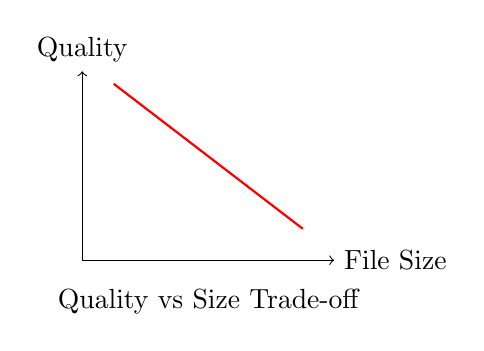
\begin{tikzpicture}[scale=0.8]
    \draw[->] (0,0) -- (4,0) node[right] {File Size};
    \draw[->] (0,0) -- (0,3) node[above] {Quality};
    \draw[thick, color=red] (0.5,2.8) -- (3.5,0.5);
    \node[below] at (2,-0.3) {Quality vs Size Trade-off};
\end{tikzpicture}
\end{center}

\end{columns}
\end{frame}

% Lossless Compression Slide
\begin{frame}{Lossless Compression - Perfect Reconstruction Methods}
\begin{columns}[T]
\column{0.6\textwidth}
\begin{alertblock}{\highlight{Lossless Compression Principles}}
Lossless compression achieves \textbf{perfect reconstruction} by exploiting statistical redundancy without discarding information.
\end{alertblock}

\textbf{Huffman Coding:}
\begin{itemize}
    \item Principle: Variable-length codes based on frequency
    \item Algorithm: Build binary tree from symbol probabilities
    \item Efficiency: Optimal for symbol-by-symbol coding
    \item Applications: JPEG (AC coefficients), PNG
    \item Limitation: Requires probability knowledge
\end{itemize}

\textbf{LZW (Lempel-Ziv-Welch):}
\begin{itemize}
    \item Principle: Dictionary-based pattern matching
    \item Algorithm: Build dictionary during encoding
    \item Advantage: Adaptive, no prior knowledge needed
    \item Applications: GIF, TIFF, PostScript
    \item Performance: Good for images with patterns
\end{itemize}

\column{0.4\textwidth}
\textbf{Run-Length Encoding (RLE):}
\begin{itemize}
    \item Principle: Replace repeated values with count
    \item Example: AAABBBBCC $\rightarrow$ 3A4B2C
    \item Efficiency: Excellent for binary images
    \item Applications: BMP, PCX, some TIFF variants
\end{itemize}

\textbf{Other Methods:}
\begin{itemize}
    \item \textbf{Arithmetic Coding}: Better than Huffman
    \item \textbf{DEFLATE}: LZ77 + Huffman (PNG)
    \item \textbf{LZMA}: Advanced dictionary compression
\end{itemize}

\vspace{0.5cm}
\begin{center}
\begin{tcolorbox}[colback=lightgray,colframe=steelblue,width=0.9\textwidth,center,boxrule=1pt]
\centering
\textbf{Perfect quality preservation}\\
\textit{Moderate compression ratios}
\end{tcolorbox}
\end{center}

\end{columns}
\end{frame}

% Huffman Encoding Demonstration
\begin{frame}{Huffman Encoding - Algorithm Demonstration}
\begin{center}

\includegraphics[width=0.85\textwidth]{images/huffman_encoding_demo.png}
\end{center}

\vspace{0.3cm}
\textbf{Key Benefits:}
\begin{itemize}
    \item \textbf{Optimal}: Minimizes average code length for given symbol frequencies
    \item \textbf{Variable Length}: Frequent symbols get shorter codes
    \item \textbf{Prefix-Free}: No code is prefix of another (unambiguous decoding)
\end{itemize}
\end{frame}

% Huffman Encoding Step-by-Step
\begin{frame}{Huffman Encoding - Complete Procedure}
\begin{center}

\includegraphics[width=0.95\textwidth]{images/huffman_procedure_steps.png}
\end{center}
\end{frame}

% Run Length Encoding Demonstration
\begin{frame}{Run Length Encoding - Simple but Effective}
\begin{center}

\includegraphics[width=0.85\textwidth]{images/rle_encoding_demo.png}
\end{center}

\vspace{0.3cm}
\textbf{Best Applications:}
\begin{itemize}
    \item \textbf{Binary Images}: Excellent compression for text, line art
    \item \textbf{Simple Graphics}: Images with large uniform areas
    \item \textbf{Preprocessing}: Often combined with other algorithms
    \item \textbf{Fax Machines}: Standard for document transmission
\end{itemize}
\end{frame}

% Lossy Compression Slide
\begin{frame}{Lossy Compression - Quality vs Size Optimization}
\begin{columns}[T]
\column{0.6\textwidth}
\begin{alertblock}{\highlight{Lossy Compression Philosophy}}
Lossy compression achieves \textbf{high compression ratios} by permanently removing information that has \textbf{minimal perceptual impact}.
\end{alertblock}

\textbf{Transform-Based Compression:}
\begin{itemize}
    \item \textbf{DCT (Discrete Cosine Transform)}: JPEG standard
    \item Principle: Convert spatial to frequency domain
    \item 8$\times$8 Blocks: Process image in small segments
    \item Quantization: Remove high-frequency components
    \item Entropy Coding: Huffman encode remaining data
\end{itemize}

\textbf{Wavelet-Based Compression:}
\begin{itemize}
    \item \textbf{JPEG 2000}: Modern wavelet standard
    \item Multi-resolution: Analyze multiple scales
    \item Better Quality: Less blocking artifacts
    \item Progressive: Quality/resolution scalability
    \item Applications: Medical, satellite imagery
\end{itemize}

\column{0.4\textwidth}
\textbf{Quantization Strategies:}
\begin{itemize}
    \item \textbf{Uniform}: Equal step sizes
    \item \textbf{Non-uniform}: Perceptually-based steps
    \item \textbf{Adaptive}: Content-dependent adjustment
\end{itemize}

\textbf{Advantages:}
\begin{itemize}
    \item High compression ratios
    \item Adjustable quality
    \item Suitable for photos
\end{itemize}

\textbf{Disadvantages:}
\begin{itemize}
    \item Irreversible loss
    \item Compression artifacts
    \item Quality degradation
\end{itemize}

\vspace{0.5cm}
\begin{center}
\textcolor{steelblue}{\textbf{Trade-off: File size vs Visual quality}}
\end{center}

\end{columns}
\end{frame}

% DCT Demonstration Slide
\begin{frame}{DCT (Discrete Cosine Transform) - JPEG Foundation}
\begin{center}

\includegraphics[width=0.95\textwidth]{images/dct_demonstration.png}
\end{center}

\vspace{0.3cm}
\textbf{DCT Process Steps:}
\begin{itemize}
    \item \textbf{Spatial → Frequency}: Transform 8×8 pixel blocks to frequency domain
    \item \textbf{Energy Compaction}: Most energy concentrated in low frequencies (top-left)
    \item \textbf{Quantization}: Remove high-frequency details (human vision less sensitive)
    \item \textbf{Reconstruction}: Inverse DCT with some information loss
\end{itemize}
\end{frame}

% Advanced Compression Slide
\begin{frame}{Advanced Compression Algorithms - Performance Analysis}
\begin{columns}[T]
\column{0.6\textwidth}
\begin{alertblock}{\highlight{Modern Compression Standards}}
Contemporary image compression algorithms balance \textbf{compression efficiency}, \textbf{computational complexity}, and \textbf{visual quality} for specific applications.
\end{alertblock}

\textbf{Next-Generation Formats:}
\begin{itemize}
    \item \textbf{WebP}: Google's VP8-based format
    \item \textbf{HEIF}: High Efficiency (H.265-based)
    \item \textbf{AVIF}: AV1-based open standard
    \item \textbf{JPEG XL}: Latest JPEG committee standard
\end{itemize}

\textbf{Performance Metrics Comparison:}
\begin{itemize}
    \item Compression Ratio: AVIF > HEIF > WebP > JPEG
    \item Quality (SSIM): JPEG XL > AVIF > HEIF > WebP
    \item Encode Speed: JPEG > WebP > HEIF > AVIF
    \item Decode Speed: JPEG > WebP > HEIF > AVIF
    \item Browser Support: JPEG > WebP > AVIF > HEIF
\end{itemize}

\column{0.4\textwidth}
\textbf{Specialized Applications:}
\begin{itemize}
    \item \textbf{Medical Imaging}: JPEG-LS, JPEG 2000 (lossless)
    \item \textbf{Satellite Data}: Custom wavelets, CCSDS standards
    \item \textbf{Mobile Photography}: HEIF with computational photography
\end{itemize}

\textbf{Future Trends:}
\begin{itemize}
    \item AI-based compression
    \item Perceptual quality metrics
    \item Real-time optimization
    \item Edge computing integration
\end{itemize}

\vspace{0.5cm}
\begin{center}
\textcolor{steelblue}{\textbf{Evolution continues: Better quality at smaller sizes}}
\end{center}

\end{columns}
\end{frame}

% Real-World Applications Slide
\begin{frame}{Real-World Applications \& Industry Case Studies}
\begin{columns}[T]
\column{0.5\textwidth}
\textbf{Medical Imaging Systems:}
\begin{itemize}
    \item \textbf{DICOM Standard}: JPEG-LS, JPEG 2000 lossless
    \item Requirements: No diagnostic information loss
    \item Storage: Petabytes of patient data
    \item Transmission: PACS networks, telemedicine
    \item Example: 16-bit CT scans, 12-bit X-rays
\end{itemize}

\textbf{Social Media Platforms:}
\begin{itemize}
    \item \textbf{Facebook}: WebP for web, HEIF mobile uploads
    \item \textbf{Instagram}: Aggressive JPEG compression with AI enhancement
    \item \textbf{TikTok}: H.264 video, JPEG thumbnails
    \item Challenges: Billions of images, mobile bandwidth
    \item Innovation: Neural super-resolution post-processing
\end{itemize}

\column{0.5\textwidth}
\textbf{E-commerce \& Product Photography:}
\begin{itemize}
    \item \textbf{Amazon}: Multi-format delivery (WebP, JPEG, AVIF)
    \item Requirements: Fast loading, zoom capability
    \item Progressive Loading: Low-quality $\rightarrow$ high-quality
    \item Mobile Optimization: Responsive images, lazy loading
\end{itemize}

\textbf{Scientific \& Satellite Imagery:}
\begin{itemize}
    \item \textbf{NASA}: Custom wavelets, lossless compression
    \item \textbf{Google Earth}: Multi-resolution pyramids
    \item \textbf{Weather Services}: Real-time compression for radar
\end{itemize}

\end{columns}

\vspace{0.5cm}
\begin{center}
\begin{tcolorbox}[colback=steelblue,colframe=steelblue,width=0.8\textwidth,center,boxrule=1pt]
\centering
\textcolor{white}{\textbf{Compression enables the digital imaging revolution}}\\
\textcolor{white}{\textit{From medical diagnosis to social media}}
\end{tcolorbox}
\end{center}

\end{frame}

% Summary Slide
\begin{frame}{Course Summary - Key Takeaways \& Future Outlook}
\begin{columns}[T]
\column{0.6\textwidth}
\begin{alertblock}{\highlight{What We've Learned Today}}
Comprehensive understanding of digital image representation, storage formats, and compression techniques that form the foundation of modern digital imaging.
\end{alertblock}

\textbf{Core Concepts Mastered:}
\begin{itemize}
    \item \textbf{Image Types}: Binary, grayscale, color, indexed representations
    \item \textbf{Storage Formats}: BMP, JPEG, PNG, GIF, TIFF characteristics
    \item \textbf{Color Models}: RGB, YUV, color space conversions
    \item \textbf{Compression}: Lossless vs lossy trade-offs and algorithms
\end{itemize}

\textbf{Critical Decision Framework:}
\begin{itemize}
    \item Quality Requirements: Medical = lossless, Web = acceptable loss
    \item Storage Constraints: Mobile vs server storage capabilities
    \item Processing Power: Real-time vs offline compression
    \item Compatibility: Universal support vs cutting-edge efficiency
\end{itemize}

\column{0.4\textwidth}
\textbf{Practical Guidelines:}
\begin{itemize}
    \item \textbf{Photography}: JPEG for sharing, RAW+lossless for archival
    \item \textbf{Graphics/Logos}: PNG for transparency, SVG for scalability
    \item \textbf{Web Development}: Progressive enhancement (AVIF$\rightarrow$WebP$\rightarrow$JPEG)
    \item \textbf{Scientific Data}: Always preserve original, compress copies
\end{itemize}

\vspace{0.5cm}
\begin{center}
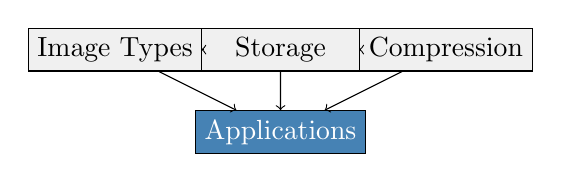
\begin{tikzpicture}[scale=0.7]
    \node[draw, rectangle, fill=lightgray, minimum width=2cm] (types) at (0,0) {Image Types};
    \node[draw, rectangle, fill=lightgray, minimum width=2cm] (storage) at (3,0) {Storage};
    \node[draw, rectangle, fill=lightgray, minimum width=2cm] (compression) at (6,0) {Compression};
    \node[draw, rectangle, fill=steelblue, text=white, minimum width=2cm] (apps) at (3,-1.5) {Applications};

    \draw[->] (types) -- (storage);
    \draw[->] (storage) -- (compression);
    \draw[->] (types) -- (apps);
    \draw[->] (storage) -- (apps);
    \draw[->] (compression) -- (apps);
\end{tikzpicture}
\end{center}

\end{columns}

\vspace{0.5cm}
\begin{center}
\begin{tcolorbox}[colback=lightgray,colframe=navyblue,width=0.8\textwidth,center,boxrule=1pt]
\centering
\textbf{\Large Questions \& Discussion}\\
\textit{From Theory to Real-World Applications}
\end{tcolorbox}
\end{center}

\end{frame}

\end{document}